\subsubsection{Tracking}
\label{subsec:03tracking}
Die zuvor beschriebene Detektion ben�tigt einen gr��eren Rechenaufwand und somit Rechenzeit, weshalb sie aufgrund der begrenzten Hardwareressourcen nicht regelm\"a{\ss}ig durchgef\"uhrt werden kann. Aus diesem Grund wird in der zweiten Phase der Personenverfolgung zum Tracking �bergegangen. \\
Tracking ist ein Vorgehen um Objekte, im vorliegenden Fall eine Person, in einer Folge von Bildern zu verfolgen. Der Vorteil ist die rechensparsame Berechnung der n\"achsten Position eines Objekts, die unter gewissen Bedingungen sogar robuster als eine Detektion sein kann. Jedoch muss Tracking zu Beginn initialisiert werden, das in diesem Fall durch die Bounding-Box der Detektion bereits gegeben ist. Zur Umsetzung des Trackings existieren verschiedene Ans\"atze, die einzelne Pixel, einen ganzen Bildteil oder Bewegungen im Bild nutzen. \\
Eine Auswahl an f\"unf Trackern wurde bereits in der OpenCV-Tracking API implementiert, sodass mehrere Tracker f\"ur die gegebene Anwendung getestet wurden. Die Tracker verwenden jeweils die interne Representation einer Bounding-Box und lernen, abgesehen vom Median Flow, einen Klassifizierer mithilfe von Online Learning\footnote{https://www.learnopencv.com/object-tracking-using-opencv-cpp-python/}. Als geeignetester Tracker stellte sich bei der Versuchsreihe der Median Flow heraus. Er bietet den besten Tradeoff zwischen Rechenzeit und Robustheit bei der Personenverfolgung. Die relativ langsamen und vorhersagbaren Bewegungen einer Person eignen sich gut f\"ur den gew\"ahlten Tracker. \\
Der Median Flow besteht aus zwei Hauptkomponenten. Im ersten Schritt wird die Bewegung ausgew\"ahlter Pixel mithilfe des Lucas-Kanade-Trackers \cite{lucaskanade} berechnet und anschlie{\ss}end wird die berechnete Position durch den Forward/Backward-Error \cite{forbackerror} evaluiert. Die beiden Komponenten werden im Folgenden genauer beschrieben:
\paragraph{Lucas-Kanade-Tracker}
Der Lucas-Kanade-Tracker basiert auf dem Prinzip des Optischen Flusses \cite{opticalflow}. So kann in einer Bildfolge die neue Position eines Pixels mit dem Zusammenhang
\begin{align}
I(x,y,t)=I(x+\text{d}x,y+\text{d}y,t+\text{d}t)
\end{align}
ausgedr\"uckt werden.
Hierbei beschreibt $I(x,y,t)$ die Intensit\"at eines Pixels an der Position $(x,y)$ zum Zeitpunkt $t$. Durch die Linearisierung mithilfe der Taylorreihenentwicklung ergibt sich die Formel des Optischen Flusses zu
\begin{align}
I_{x}u+I_{y}v+I_{t} = 0 
\end{align}
mit 
\begin{align}
u=\frac{\text{d}x}{\text{d}t},\ v=\frac{\text{d}y}{\text{d}t},\ I_{x}=\frac{\text{d}I}{\text{d}x},\ I_{y}=\frac{\text{d}I}{\text{d}y},\ I_{t}=\frac{\text{d}I}{\text{d}t}.
\end{align}
Nun besteht die Aufgabe die Bewegeung $(u,v)$ zu bestimmen. Dies wird mithilfe einer Erweiterung der Gleichung unter Einbeziehung der benachbarten Pixel in einem $3x3$ Fenster erm\"oglicht. Damit ergibt sich
\begin{align}
\begin{pmatrix}
I_{x}(p_{1}) & I_{y}(p_{1}) \\ 
... & ...\\ 
I_{x}(p_{9}) & I_{y}(p_{9})
\end{pmatrix} 
\begin{pmatrix}
u\\ 
v
\end{pmatrix}+
\begin{pmatrix}
I_{t}(p_{1})\\ 
...\\ 
I_{t}(p_{9})
\end{pmatrix} = 0
\end{align}
als erweiterter Zusammenhang.
Die \"uberbestimmte Formel beinhaltet die 9 Pixel $p_{1}...p_{9}$ aus dem $3x3$ Fenster und kann mithilfe der Methode der kleinsten Quadrate gel\"ost werden. Als Ergebnis wird die Bewegung eines Pixels, die die Verfolgung �ber eine Folge von Bildern erm\"oglicht, erhalten.
\paragraph{Forward/Backward Error}
Der Lucas-Kanade-Tracker verfolgt ein Pixel �ber eine Bilderfolge von $k$ Bildern,sodass eine Trajektorie $T^{k}_{f}=(x_{t},x_{t+1},...,x_{t+k})$ bestimmt werden kann. Hierbei steht $f$ f\"ur forward und beschreibt die Forw\"artstrajektorie. Das Ziel ist nun, diese Trajektorie zu validieren. Hierf�r wird bei der Position $x_{t+k}$ begonnen und dieses Pixel r\"uckw\"arts �ber die gegebene Folge von $k$ Bildern verfolgt. So wird eine zweite Trajektorie $T^{k}_{b}=(\hat{x}_{t},\hat{x}_{t+1},...,\hat{x}_{t+k})$ bestimmt, die mit der ersten verglichen wird. Um die Berechnung simpel zu halten, wird die euklidische Distanz
\begin{align}
\text{distance}(T^{k}_{f},T^{k}_{b})= \left \| x_{t} - \hat{x}_{t} \right \|
\end{align} 
zwischen Start und Endpunkt der jeweiligen Trajektorie als Vergleichsoperator gew�hlt.
In Abbildung \ref{fig:ForBackError} wird das Vorgehen zur Bestimmung des Forward/Backward Errors nochmals veranschaulicht. \\
\begin{figure}[h]
	\centering
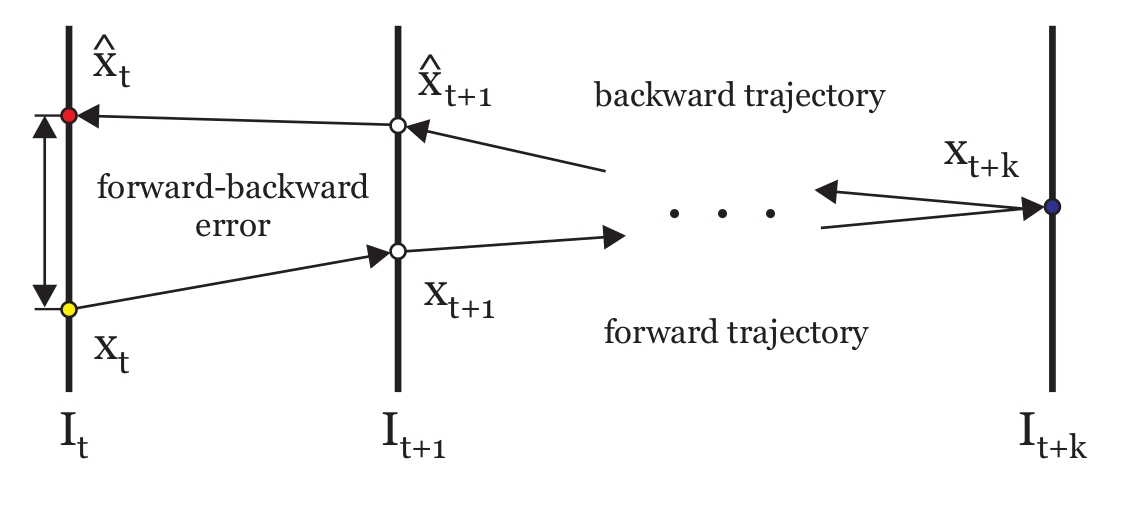
\includegraphics[width=0.6\textwidth,trim=2.4cm 0cm 0cm 1cm,clip]{pics/ForwardBackwardE.jpg}
	\caption{Das Vorgehen zur Berechnung des Forward/Backward Errors. (aus \cite{forbackerror})}
	\label{fig:ForBackError}
\end{figure} \\

Die beschriebene Methode zur Validierung wird in der Implementierung des Median Flows zwei mal angewendet. Zu Beginn wird sie zur Auswahl der Featurepunkte aus dem Detektionfenster, die mit dem Ansatz von Lucas und Kanade getrackt werden sollen, genutzt. So werden die Pixel verworfen, die einen hohen Forward/Backward Error aufweisen und die signifikanten f�r Tracking geeigneten Features behalten. Weiterhin wird der Fehler zur Validierung des gesamten Trackingergebnisses genutzt und erm�glicht die Erkennung eines fehlerhaften Trackings.